\chapter{Deep Learning}

\section{Introducción}
% The basic unit is the so-called neuron
% I A Linear Discriminant Function (LDF)
% I With an activation function

\begin{paracol}{2}
   La unidad basica es el llamado \textbf{neuron}, que implementa una \textit{Función Discriminante Lineal} (\textsc{LDF}) con una función de activación. Un neurón recibe múltiples entradas, aplica pesos a estas entradas, suma los resultados y pasa esta suma a través de una función de activación para producir una salida.
   
   \switchcolumn

   \begin{figure}[htbp]
      \centering
      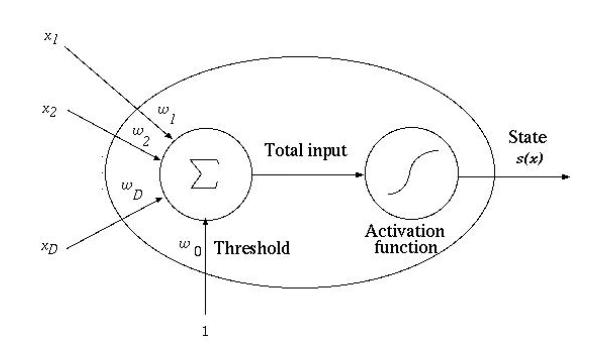
\includegraphics{images/08/neuron.png}
      \caption{Neuron}
      \label{fig:08/neuron}
   \end{figure}

\end{paracol}

Matemáticamente, un neurón se puede representar como:

\[ y = f\left(\sum_{i=1}^{n} w_i x_i + b\right) \]

Donde:
\begin{itemize}
   \item $x_i$ son las entradas
   \item $w_i$ son los pesos
   \item $b$ es el sesgo (bias)
   \item $f$ es la función de activación
\end{itemize}

Neurones pueden ser combinados en \textsc{capas} (\textit{layers}): lineal layers, convolutional layers, recurrent layers, etc.
Capas pueden ser combinados en redes neuronales (\textit{neural networks}).

\begin{figure}[htbp]
   \centering
   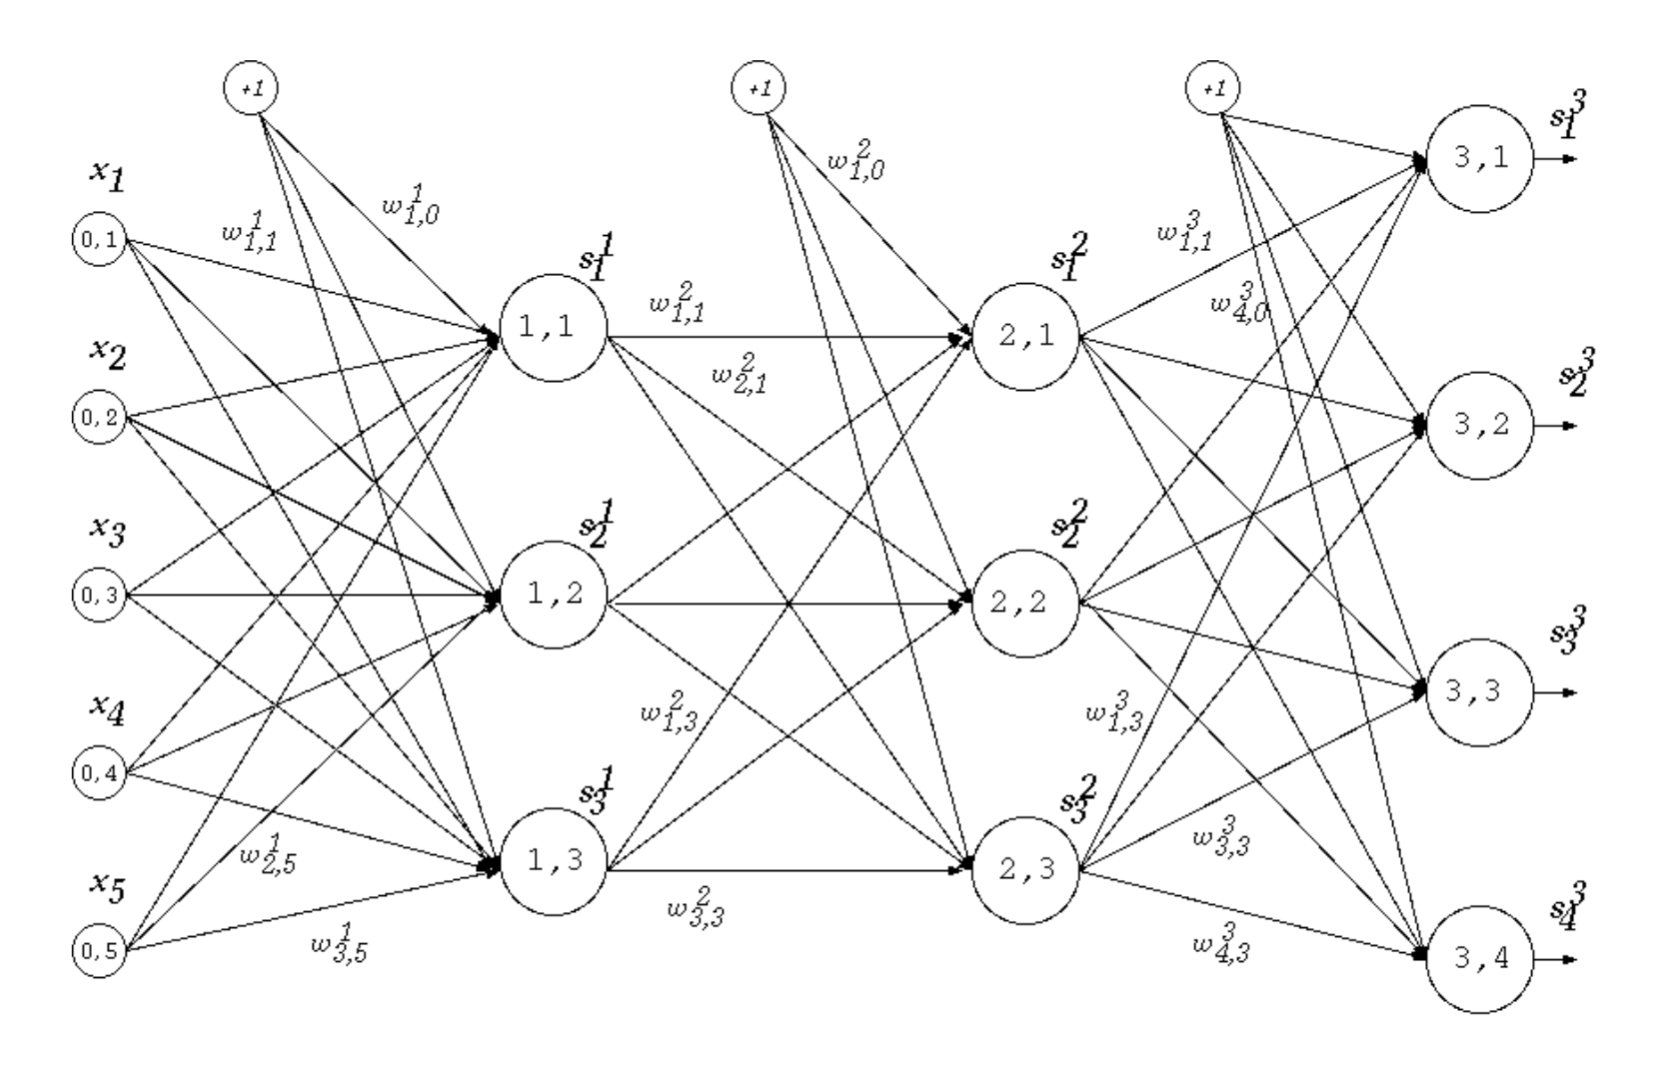
\includegraphics{images/08/layers1.png}
   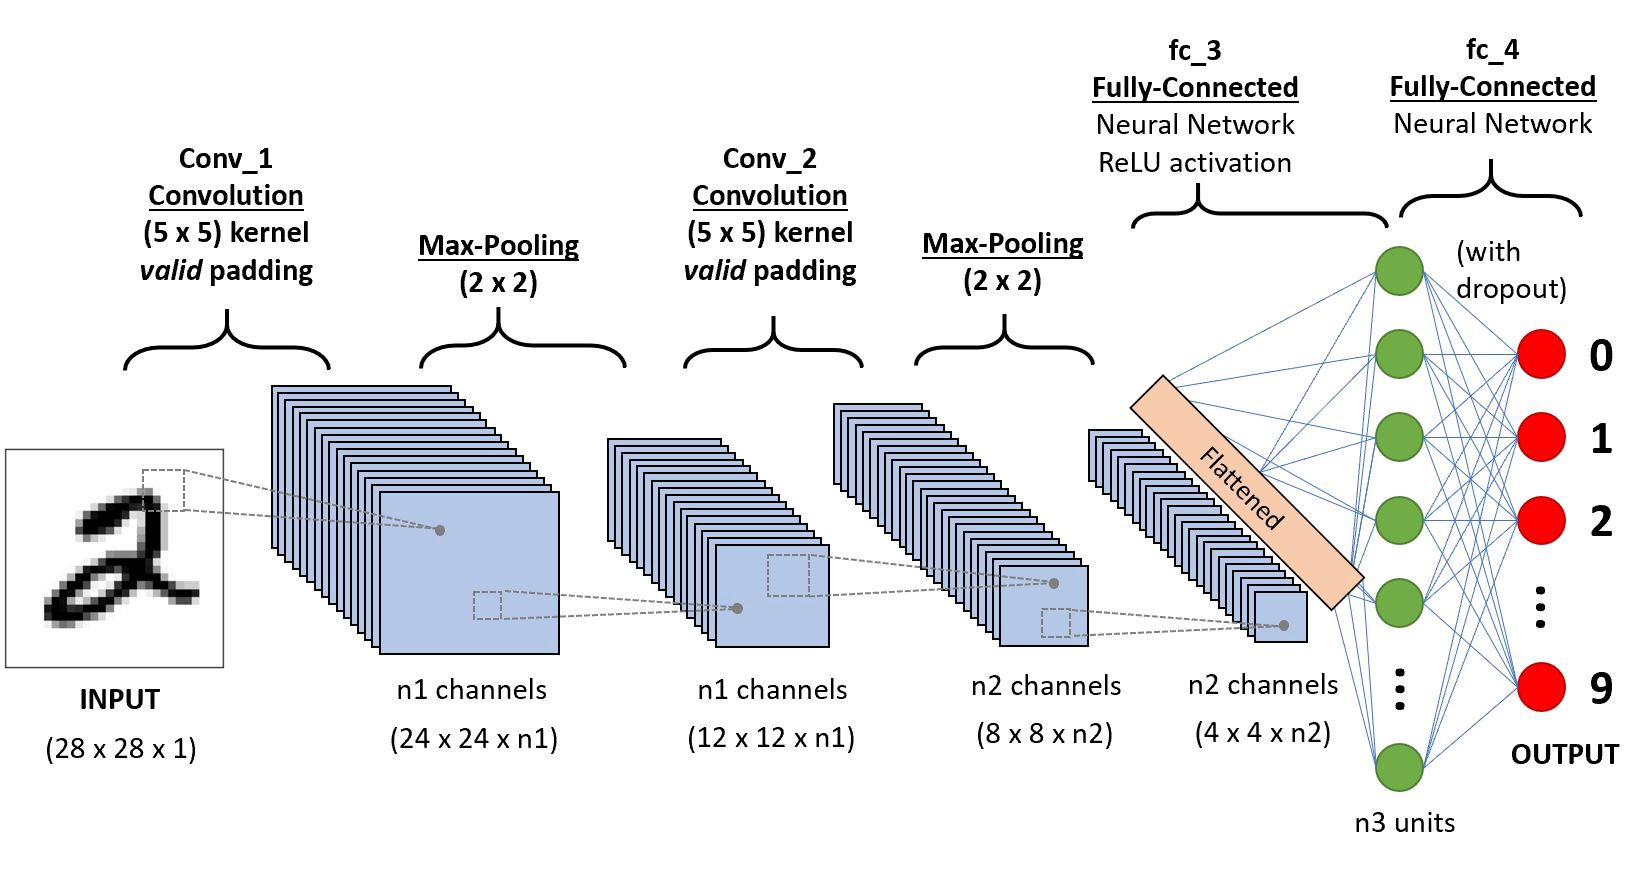
\includegraphics{images/08/layers2.jpeg}
   \caption{Capas y redes neuronales}
   \label{fig:08/layers}
\end{figure}

\newpage
\section{Linear Discriminant Function and Perceptron}

A classifier $G$ in $C$ classes can be defined by $C$ discriminant functions $g_c$.\\
Classification rule $(\vec{x} \in \mathbb{R}^D ): \hat{c} = G(\vec{x}) = arg max_{c=1},...,C g_c (\vec{x})$

\begin{figure}[htbp]
   \centering
   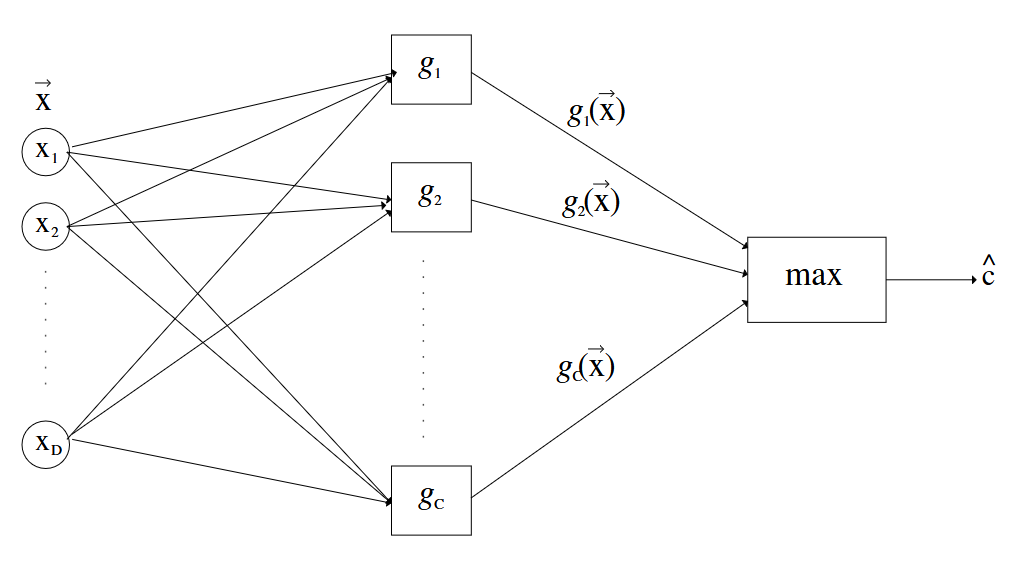
\includegraphics{images/08/discriminant.png}
   \caption{Discriminant function Graph}
   \label{fig:08/discriminant}
\end{figure}

When $g_c$ are linear functions, they are called \textbf{Linear Discriminant Functions} (\textsc{LDF})
\[
   g(\vec{x}) = w0 + \sum^D_{i=1}\vec{w_i} \vec{x_i} = w0 + \vec{w^t} \vec{x}
   \]
$\vec{w}$ is the weights vector, w0 is the bias term
In homogeneus notation: $w = (w0, \vec{w^t} )t , x = (1, \vec{x^t} )t$
\[g(\vec{x}) = w^t x\]
G is a linear classifier when all $g_c$ are linear functions, with parameters $w_c$
Given a training dataset of samples in $\mathbb{R}^D$, $w_c$ can be estimated by \ul{using the
\textbf{Perceptron} algorithm}

\begin{figure}[htbp]
   \centering
   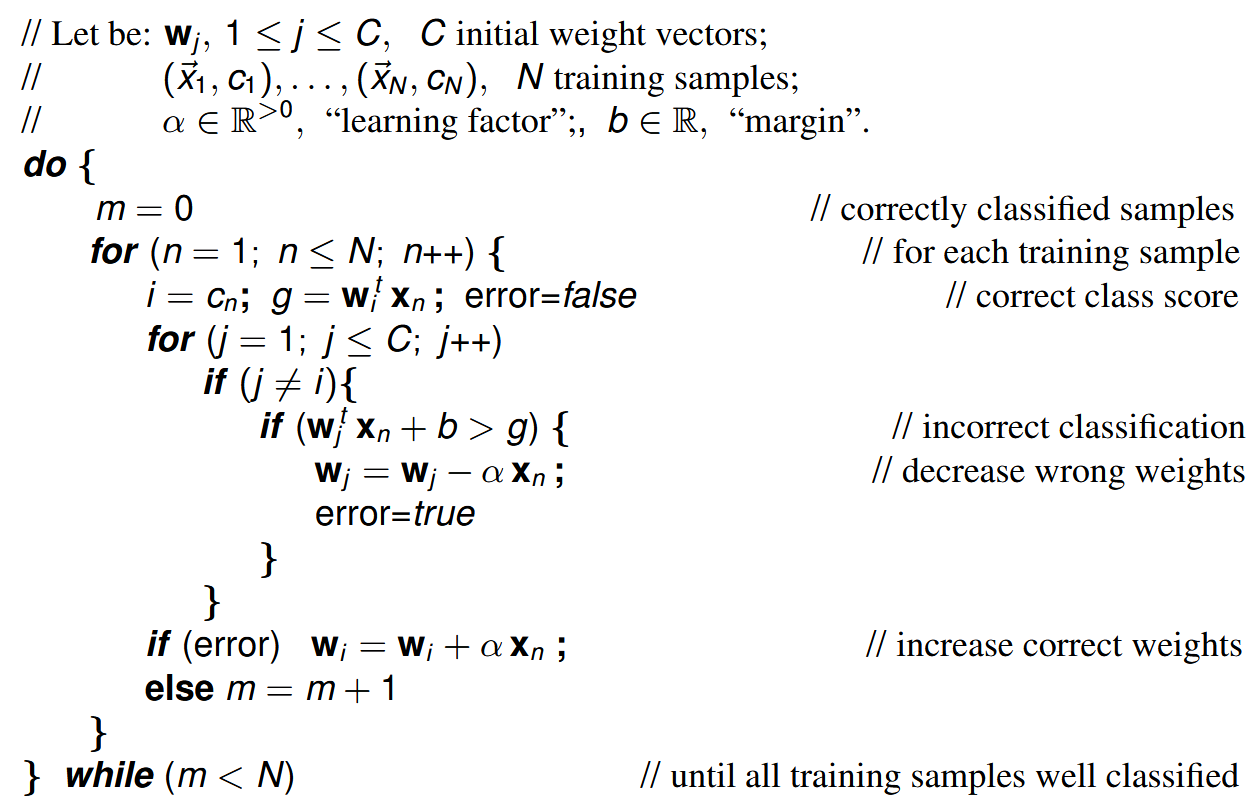
\includegraphics{images/08/perceptron.png}
   \caption{Perceptron algorithm}
   \label{fig:08/perceptron}
\end{figure}

% \begin{algorithm}
%    \caption{Perceptron algorithm}\label{euclid}
%    \begin{algorithmic}[1]
%       \State Perceptron algorithm
%       \State // Let be: $w_j , 1 \leq j \leq C, C$ initial weight vectors;
%       \State // $(\vec{x_1}, c_1), \dots , (\vec{x_N} , c_N ), N  $ training samples;
%       \State // $\alpha \in \mathbb{R}>0, ``learning factor'', b \in \mathbb{R}$, ``margin''.
%       % \Procedure{MyProcedure}{}
%       % \EndProcedure
%    \end{algorithmic}
% \end{algorithm}

\newpage
The main limitation is that LDF provide linear frontiers only linearly separable classes
can be properly separated.
Using margin b allows for a non-optimal solution
Combining several LDF in cascade does not solve the problem:
result is still an LDF.\\
\ul{Solution: use of \textit{Activation Functions}} $\rightarrow$ \textbf{Logistic LDF} (neuron).

\begin{figure}[htbp]
   \centering
   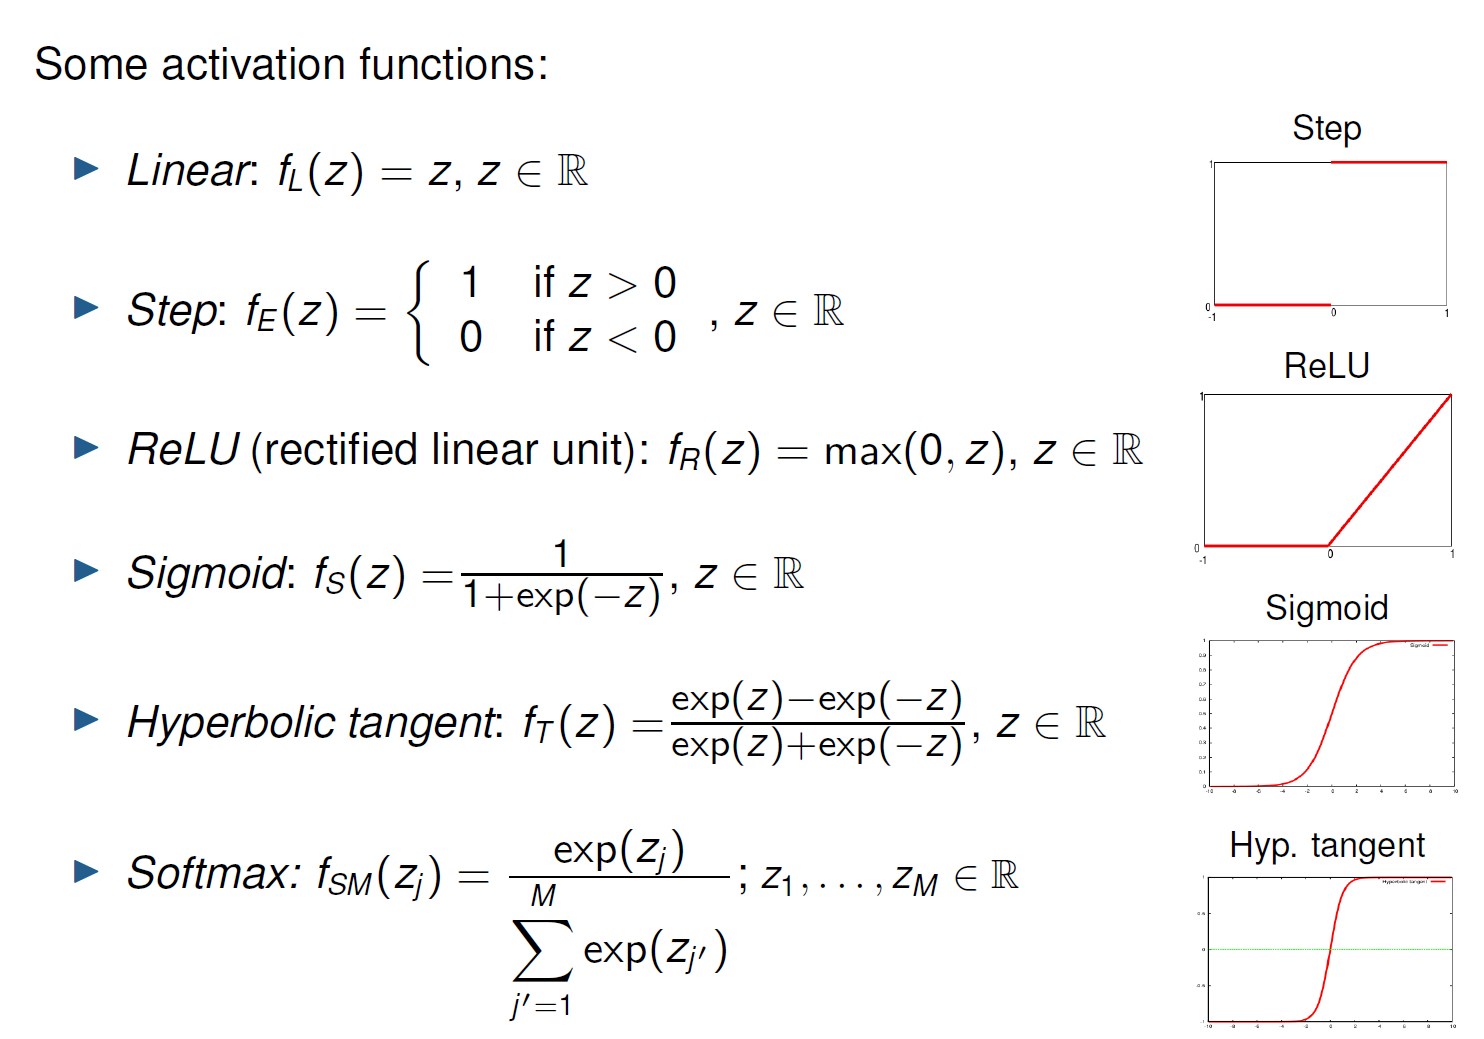
\includegraphics{images/08/activation.png}
   \caption{Activation Functions}
   \label{fig:08/activation}
\end{figure}


\subsection{Backpropagation}

The \textbf{Backpropagation} algorithm is used to train neural networks by minimizing the error between the predicted output and the actual output. It works by calculating the gradient of the loss function with respect to each weight in the network, allowing for efficient weight updates.

\begin{figure}[htbp]
   \centering
   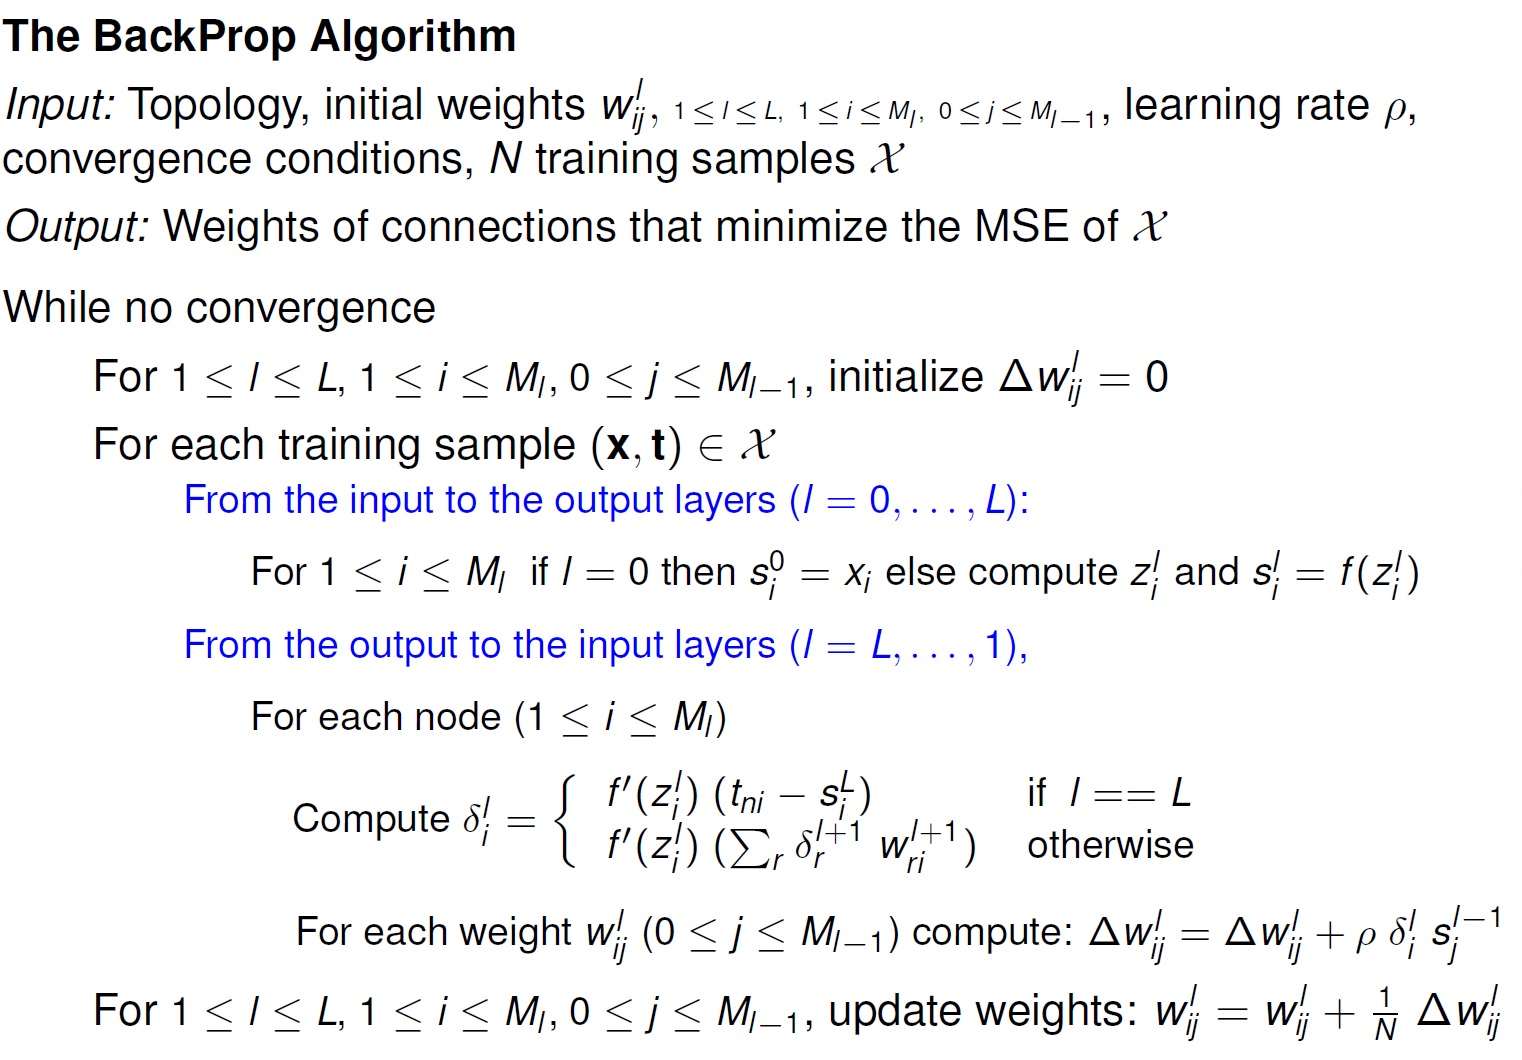
\includegraphics{images/08/backprop.png}
   \caption{Backpropagation Algorithm}
   \label{fig:08/backprop}
\end{figure}

\newpage
\begin{algorithm}
\caption{BackProp Algorithm}
\begin{algorithmic}[1]
\State \textbf{Input:} Topology, initial weights $w_{ij}^l, 1 \leq l \leq L, 1 \leq i \leq M_l, 0 \leq j \leq M_{l-1}$; learning rate $\rho$; convergence conditions; $N$ training samples $\mathcal{X}$
\State \textbf{Output:} Weights that minimize the MSE of $\mathcal{X}$

\While{no convergence}
    \For{$1 \leq l \leq L$, $1 \leq i \leq M_l$, $0 \leq j \leq M_{l-1}$}
        \State Initialize $\Delta w_{ij}^l = 0$
    \EndFor

    \For{each training sample $(\mathbf{x}, \mathbf{t}) \in \mathcal{X}$}
        \Comment \textcolor{blue}{From input to output layers $(l = 0, \dots, L)$}
        \For{$1 \leq i \leq M_l$}
            \If{$l == 0$}
                \State $s_i^0 = x_i$
            \Else
                \State Compute $z_i^l$ and $s_i^l = f(z_i^l)$
            \EndIf
        \EndFor

        \Comment \textcolor{blue}{From output to input layers $(l = L, \dots, 1)$}
        \For{each node $1 \leq i \leq M_l$}
            \If{$l == L$}
                \State $\delta_i^l = f'(z_i^l)(t_{ni} - s_i^L)$
            \Else
                \State $\delta_i^l = f'(z_i^l)\left( \sum_r \delta_r^{l+1} w_{ri}^{l+1} \right)$
            \EndIf
        \EndFor

        \For{each weight $w_{ij}^l$ ($0 \leq j \leq M_{l-1}$)}
            \State $\Delta w_{ij}^l = \Delta w_{ij}^l + \rho \, \delta_i^l s_j^{l-1}$
        \EndFor
    \EndFor

    \For{$1 \leq l \leq L$, $1 \leq i \leq M_l$, $0 \leq j \leq M_{l-1}$}
        \State Update weights: $w_{ij}^l = w_{ij}^l + \frac{1}{N} \Delta w_{ij}^l$
    \EndFor
\EndWhile

\end{algorithmic}
\end{algorithm}

\subsection{Resumen del algoritmo de Backpropagation}

El algoritmo de Backpropagation (retropropagación) es fundamental para el entrenamiento de redes neuronales y funciona de la siguiente manera:

\begin{enumerate}
    \item \textbf{Inicialización:} Se parte de una topología de red definida con pesos iniciales aleatorios, una tasa de aprendizaje y un conjunto de datos de entrenamiento.
    
    \item \textbf{Ciclo principal:} Se itera hasta alcanzar la convergencia (cuando el error es suficientemente pequeño o se alcanza un número máximo de iteraciones).
    
    \item \textbf{Para cada ciclo:}
    \begin{itemize}
        \item Se inicializan los cambios de pesos a cero.
        \item Para cada muestra de entrenamiento:
        \begin{itemize}
            \item \textbf{Propagación hacia adelante (forward pass):} Se calcula la salida de la red, capa por capa, desde la entrada hasta la salida.
            \item \textbf{Propagación hacia atrás (backward pass):} Se calcula el error en la capa de salida y se propaga hacia atrás, calculando los deltas (errores) para cada neurona en cada capa.
            \item Se acumulan los cambios necesarios para cada peso basados en los deltas calculados y las activaciones previas.
        \end{itemize}
        \item Se actualizan todos los pesos usando el promedio de los cambios calculados para todas las muestras.
    \end{itemize}
\end{enumerate}

La clave del algoritmo está en la regla de la cadena del cálculo diferencial, que permite calcular eficientemente cómo contribuye cada peso al error total de la red, facilitando así su actualización en la dirección que reduce dicho error.


Para la clasificación $J$ se utiliza la Cross-Entropy Loss Function:
\[
C_\chi = -\frac{1}{N}\sum_{n=1}^{N} \sum_{c=1}^{C} t_{nc} \log s_c^L(\mathbf{x_n};\mathbf{w})
\]

La convergencia depiende de la tasa de aprendizaje $\rho$ y del número de iteraciones $N$.
\begin{itemize}
   \item  Si $\rho$ es muy grande, la convergencia puede ser inestable y oscilar.
   \item Si $\rho$ es muy pequeña, la convergencia puede ser muy lenta
   \item $\rho = 2/(\delta_{max} + \delta_{min})$ es una buena aproximación, donde $\delta_{max}$ y $\delta_{min}$ son los valores máximos y mínimos de los deltas.
   Garantiza convergencia asymptoticamente.
\end{itemize}